\documentclass[a4paper]{article}
\usepackage[utf8]{inputenc}
\usepackage[english]{babel}
\usepackage{enumitem}	%enumerate
\usepackage{fancyhdr}	%intestazioni e piè pagina
\fancypagestyle{SE2}{% Software Engineering 2 Project Page Style
	\pagestyle{fancy}	
	%\fancyhead[LE,RO]{\slshape\rightmark}
	%\fancyhead[LO,RE]{\slshape\leftmark}
	%\fancyhead[L,R]{\slshape\rightmark}
	\cfoot{} % get rid of the page number 
	\fancyfoot[L]{\emph{PowerEnJoy}\quad \textbf{R}equirement \textbf{A}nalysis and \textbf{S}pecifications \textbf{D}ocument}
	\fancyfoot[R]{\thepage}
	\renewcommand{\headrulewidth}{0.4pt}
	\renewcommand{\footrulewidth}{0.4pt}
}
\pagestyle{SE2}
%\pagestyle{fancy}
\usepackage{graphicx}	%immagini
\usepackage[colorinlistoftodos]{todonotes}	%todo
%numeri romani maiuscoli
\newcommand{\RomanNumber}[1]{\uppercase\expandafter{\romannumeral #1\relax}}
\usepackage{hyperref} %link pdf
\hypersetup{
    colorlinks,
    citecolor=black,
    filecolor=black,
    linkcolor=black,
    urlcolor=black
}
\graphicspath{{./img/}} %extra root-path for images
\usepackage[T1]{fontenc}
%\usepackage[style=alphabetic]{biblatex}
%\usepackage[babel]{csquotes}
%\usepackage[bibstyle=authortitle,citestyle=verbose-trad1]{biblatex}
%\bibliography{RASD-main.bib}
%
\usepackage[toc,page]{appendix}
\usepackage{eurosym}%\simbolo euro
\usepackage{booktabs}%table rule
\usepackage{longtable} %multiple page tables
\usepackage{listings} 
% Define Language
\lstdefinelanguage{alloy}
{
  % list of keywords
  morekeywords={
	assert, pred, all, no, lone, one, some, check, run,
      but, let, implies, not, iff, in, and, or, set, sig, Int, int,
      if, then, else, exactly, disj, fact, fun, module, abstract,
      extends, open, none, univ, iden, seq,
  },
%  literate=%
%    {:}{$\colon$}1
%    {|}{$\bullet$}1
%    {==}{$=$}1
%    {=}{$=$}1
%    {!=}{$\neq$}1
%    {&&}{$\land$}1
%    {||}{$\lor$}1
%    {<=}{$\le$}1
%    {>=}{$\ge$}1
%    {all}{$\forall$}1
%    {exists}{$\exists$}1
%    {!in}{$\not\in$}1
%    {\\in}{$\in$}1
%    {=>}{$\implies$}2
%    ,
  sensitive=true, % keywords are not case-sensitive
  morecomment=[l]{//}, % l is for line comment
  morecomment=[s]{/*}{*/}, % s is for start and end delimiter
  morestring=[b]" % defines that strings are enclosed in double quotes
}

% Define Colors
\usepackage{color}
\definecolor{eclipseBlue}{RGB}{42,0.0,255}
\definecolor{eclipseGreen}{RGB}{63,127,95}
\definecolor{eclipsePurple}{RGB}{127,0,85}
 
% Set Language
\lstset{
  language={alloy},
  basicstyle=\small\ttfamily, % Global Code Style
  captionpos=b, % Position of the Caption (t for top, b for bottom)
  extendedchars=true, % Allows 256 instead of 128 ASCII characters
  tabsize=2, % number of spaces indented when discovering a tab 
  columns=fixed, % make all characters equal width
  keepspaces=true, % does not ignore spaces to fit width, convert tabs to spaces
  showstringspaces=false, % lets spaces in strings appear as real spaces
  breaklines=true, % wrap lines if they don't fit
  frame=trbl, % draw a frame at the top, right, left and bottom of the listing
  frameround=false, % make the frame round at all four corners
  framesep=4pt, % quarter circle size of the round corners
  numbers=left, % show line numbers at the left
  numberstyle=\tiny\ttfamily, % style of the line numbers
  commentstyle=\color{eclipseGreen}, % style of comments
  keywordstyle=\color{eclipsePurple}, % style of keywords
  stringstyle=\color{eclipseBlue}, % style of strings
}

\begin{document}

\begin{titlepage}
\newcommand{\HRule}{\rule{\linewidth}{0.5mm}} % Defines a new command for the horizontal lines, change thickness here

\center % Center everything on the page
 
%----------------------------------------------------------------------------------------
%	HEADING SECTIONS
%----------------------------------------------------------------------------------------

\includegraphics[scale=0.3]{logo_poli.png}\\[0.5cm] % Include a department/university logo - this will require the graphicx package
\textsc{\LARGE Politecnico di Milano}\\[2cm] % Name of your university/college
\textsc{\Large Software Engineering \RomanNumber{2} project}\\[0.5cm] % Major heading such as course name
\textsc{\large \textbf{PowerEnJoy}}\\[1.5cm] % Minor heading such as course title

%----------------------------------------------------------------------------------------
%	TITLE SECTION
%----------------------------------------------------------------------------------------

\HRule \\[0.4cm]
{ \huge \bfseries Requirements Analysis\\ and Specifications Document}\\[0.4cm] % Title of your document
\HRule \\[1.5cm]
 
%----------------------------------------------------------------------------------------
%	AUTHORS SECTION
%----------------------------------------------------------------------------------------

\begin{minipage}{0.4\textwidth}
\begin{flushleft} \large
\emph{Authors:}\\
Davide \textsc{Piantella}\\
Mario \textsc{Scrocca}\\
Moreno R. \textsc{Vendra} % Your name
\end{flushleft}
\end{minipage}
~
\begin{minipage}{0.4\textwidth}
\begin{flushright} \large
\emph{Professor:} \\
Luca \textsc{Mottola} % Supervisor's Name
\end{flushright}
\end{minipage}\\[2cm]

% If you don't want a supervisor, uncomment the two lines below and remove the section above
%\Large \emph{Author:}\\
%John \textsc{Smith}\\[3cm] % Your name

%----------------------------------------------------------------------------------------
%	DATE SECTION
%----------------------------------------------------------------------------------------

{\large December 8, 2016}\\[0.5cm] % Date, change the \today to a set date if you want to be precise
{\large version 1.3}\\[2cm]
 
%----------------------------------------------------------------------------------------

\vfill % Fill the rest of the page with whitespace
\clearpage
\end{titlepage}


%----------------------------------------------------------------------------------------
%----------------------------------------------------------------------------------------
%----------------------------------------------------------------------------------------
%----------------------------------------------------------------------------------------
%	TABLE OF CONTENTS
%----------------------------------------------------------------------------------------
\pagenumbering{Roman}
\tableofcontents
\listoffigures
\listoftables
\hypersetup{
	linkcolor=blue,
	citecolor=blue
}
%----------------------------------------------------------------------------------------
%	INTRODUCTION
%----------------------------------------------------------------------------------------
\clearpage
\pagenumbering{arabic}
\section{Introduction}
\subsection{Purpose of this document}
The purpose of a \textbf{R}equirement \textbf{A}nalysis and \textbf{S}pecifications \textbf{D}ocument is the process of discovering the purpose for which a software system was intended, by identifying stakeholders and their needs, and documenting these in a form that is amenable to analysis, communication, and subsequent implementation. \todo{Citation} It is also concerned with the relationship of software's factors such as goals, functions and constrains to precise specifications of software behavior, and to their evolution over time and across software families.

\subsection{Actual system}
The system we are to develop is brand new, there is no previous system.

\subsection{Scope}
PowerEnJoy is a car-sharing service that exclusively employs electric cars; we are going to develop a web-based software system that will provide the functionalities normally provided by car-sharing services, such as allowing the user to register to the system in order to access it, showing the cars available near a given location and allowing a user to reserve a car before picking it up.
A screen located inside the car will show in real time the ride amount of money to the user. When the user reaches a predefined safe area and exits the car, the system will stop charging the user and will lock the car. The system will provide information about charging station location where the car can be plugged after the ride and incentivize virtuous behaviours of the users with discounts.
	\subsubsection{Goals}
	\begin{enumerate}[label=\textbf{G\arabic*}]
		\item \label{goal:register} Allow users to register to the system
		\item \label{goal:login}Allow registered users to authenticate to the system
		\item \label{goal:position}Provide authenticated users with the position of available cars
		\item \label{goal:notifyMaintenance} Notify maintenance service with a list of not available cars 
		\item \label{goal:maintenanceDone} Provide the maintenance service with a way to notify the system when a car is available again 
		\item \label{goal:needMaintenance} Provide the user with a way to contact customer service to report a damaged car
		\item \label{goal:usersHistory} Provide a way to show to the user his rent and payment history and make these information accessible also to the customer service
		\item \label{goal:banUnbanUsers}Provide customer service with a way to ban users in order to prevent them from reserving or using other cars, and enable them to use the service again
		\item \label{goal:carReservation} Allow a user to reserve a car, if available, and hold that reservation for an hour
		\item \label{goal:reservationFee}Charge the user for 1\euro\ in case he hasn't used the car he reserved after an hour from such reservation
		\item \label{goal:completeRent}Allow a user to perform a complete rent: reserving a car, using it and leaving it terminating the rent, accomplishing the payment procedure related to aforementioned rent
		\item \label{goal:calculateCost}Calculate and charge the user for the correct amount of money he has to pay for his last ride, also considering the various discounts and fees applicable based on the ride
		\item \label{goal:moneySavingOption}Allow the user to enable a money saving option which provides him with a charging station as destination of the ride to get a discount on the cost of the aforementioned ride
	\end{enumerate}

\subsection{Glossary}
	\subsubsection{Definitions}
	\begin{description}
		\item[System:]the PowerEnJoy software we are to develop
		\item[Company:] the company we are developing the system for
		\item[Guest \emph{or} Guest user:] person who access the system as non logged user
		\item[Logged user \emph{or} Authenticated user:] authenticated person who is interfacing with the system
		\item[User:] \todo{only logged user? to be consistent with requirements} guest user or logged user
		\item[Banned user:] a user that can not use the system, he can only contact the customer care service
		\item[Registration:]  interaction between a non registered user and the system in which the user, providing all of the information required by the system for the creation of an account, receives from the system the credentials needed to authenticate to the system
		\item[Car:] an electric car owned by the company
		\item[Available car:] the car can be reserved by a user(i.d. the car is working correctly and its battery level is not critical)
		\item[Reserved car:] the car has been reserved by a user
		\item[In use car:] the user has ignited the car engine and he is still in the car
		\item[Not available car:] the car can not be reserved by a user (i.d. the car is not working correctly or its battery level is critical), a maintenance operator will deal with it
		\item[Battery level critical:] battery level under 20\%
		\item[Charging station:] location where cars owned by the company can be charged using a provided plug
		\item[Authentication \emph{or} Login:] interaction between guests and the system that grants authenticated user's privileges to a guest user
		\item[Safe area:] area of the map where a rent can be terminated without the corresponding additional fee
		\item[Payment procedure:] process which realizes the monetary transaction between the user and the system
		\item[Restricted access API:] API that can be used only by authorized person or system
		\item[GPS Coordinates:] GPS coordinates are a unique identifier of a precise geographic location on the earth
	\end{description}
\subsubsection{Acronyms}
	\begin{description}
		\item [RASD:] Requirements Analysis and Specification Document
		\item [API:] Application Programming Interface
		\item [GPS:] Global Position System
		\item [DBMS:] Data Base Management System
		\item [FSM:] Finite-State Machine
	\end{description}
\subsubsection{Abbreviations}
	\begin{description}
		\item [Km:] Kilometers
		\item [w.r.t.:] with respect to
		\item [i.d.:] id est
		\item [i.f.f.:] if and only if
		\item [e.g.:] exempli gratia
		\item [etc.:] et cetera
	\end{description}

\subsection{Document overview}
This document is structured in \todo{Complete, also with IEEE ref}
\begin{enumerate}
	\item \textbf{Introduction}: it provides an overview of this entire document and product goals
	\item \textbf{Overall description}: it describes general factors that affect the product providing the background for system requirements
	\item \textbf{Specific requirements}: it contains all system requirements
	\item \textbf{Use cases identification}: it contains the usage scenario of the system, the use case diagram and use cases description
	\item Appendix
\end{enumerate}

\section{Overall description}
\subsection{Product perspective}
	\subsubsection{System interfaces}
	\label{sec:systemInterfaces}
		The system we are to develop will have some external interfaces (represented in Figure \ref{fig:systemInterfaces}) to accomplish the goals stated in section 1.3.1\todo{reference?}.
		\begin{figure}[h]
			\centering
			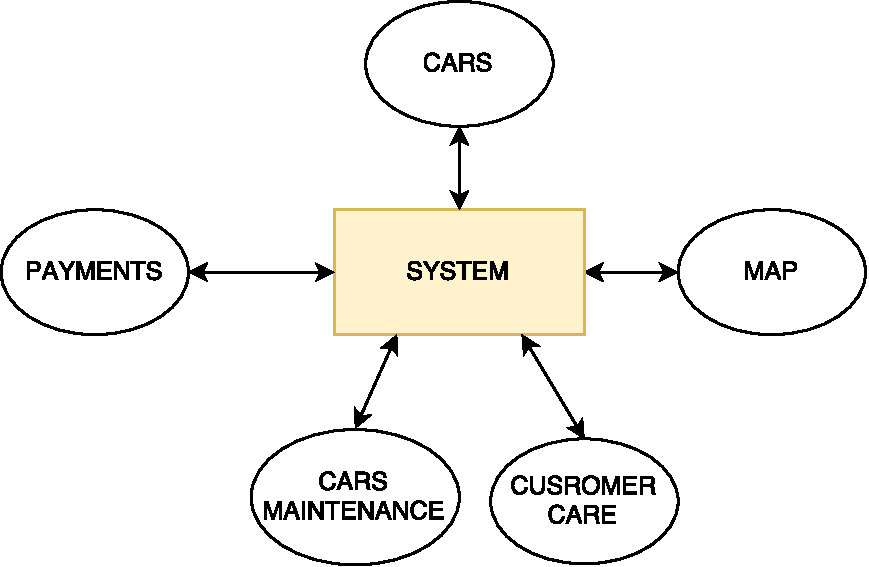
\includegraphics[scale=0.5]{system_blocks}
			\caption{
				\label{fig:systemInterfaces} 
				Overview of system interfaces
			}
		\end{figure}
	\paragraph{Payments}
	When a payment is required (e.g. when a user ends his rent) the system sends a request with all the details needed to complete the payment (i.d. name and surname of the user, due amount, credit card number etc.) to an external payment handling system. Once the external system completes the payment process, it sends our system the payment outcome so that the system can take appropriate action.
	
	\paragraph{Customer care} Every time it is required, a PowerEnJoy customer care service operator can interact with a user. Customer care service operators can request and see all user details, their rents and payments history. Such operators can also ban or unban users from the system, mark cars as not available and, in general, provide assistance to users.

	\paragraph{Maintenance} The system will interact with a preexisting car maintenance service which already deals with other car sharing services. Our system will expose to the maintenance service a real time list of all the cars tagged as \emph{not available} via a \emph{restricted access API} providing their GPS position and a brief description of the problem. The maintenance service takes care of reaching those cars, unlock the doors, \todo{in UseCase expand lock/unlock proc.} fix the fault, re-lock the doors and finally tag them as \emph{available} using the aforementioned API provided by the system.
	
	\paragraph{Map} GPS position of cars and safe areas is displayed to all users, customer care operators and maintenance operators on a constantly updated map which relies on an external Geographic Information System.

	\paragraph{Cars}\label{sec:cars}All cars provided by the customer are equipped with a communication system which ensures a continuous protected communication between the car and the system. All cars also have a module which provides a set of primitives that allow the system to retrieve information and to run commands to take actions on the car. A built-in user interface embedded with the modules shows some relevant information to the user.\\
	Information retrieved by the system from the car include:
	\begin{itemize}
		\item unique car identifier
		\item GPS position
		\item engine status (on, off)
		\item number of passengers
		\item battery level (percentage)
		\item charging status (in charge, not in charge)
		\item door locking status (locked, unlocked)
		\item system failure description, if present
	\end{itemize}
	Information sent to the car by the system include:
	\begin{itemize}
		\item location of safe areas
		\item position of charging stations
		\item current time
	\end{itemize}
	Commands runnable by the system include:
	\begin{itemize}
		\item lock doors \todo{may be useful, never used in normal event flow}
		\item unlock doors
		\item set car status (see \autoref{fig:carFSA})
	
	\end{itemize}		
	Information shown to the user by the embedded car interface include:
	\begin{itemize}
		\item current car position (also w.r.t. safe areas and charging stations)
		\item number of passengers
		\item battery level (percentage)
		\item current time
		\item amount owned until now
	\end{itemize}

	The overall status of a car can be represented by an FSM
	\begin{figure}[h]
			\centering
			\includegraphics[scale=0.5]{CarFSA}
			\caption{
				\label{fig:carFSA} 
				Car statuses
			}
		\end{figure}
		
\subsubsection{User interfaces}
	Using the interfaces of the system users can:\todo{move car to system interface}
	\begin{enumerate}
		\item Register and log-in to the system
		\item On the map they can view the position of
			\begin{enumerate}[label=\alph*)]
				\item themselves
				\item safe areas
				\item available cars (with their current battery level)
				\item charging stations
			\end{enumerate}
		\item Reserve a car
		\item Ask the customer care service for assistance 
	\end{enumerate}
%	Using the interface in the car users can:
%	\begin{enumerate}
%		\item Start the engine
%		\item View the real time battery level
%		\item View their real time GPS position
%		\item View their position w.r.t safe areas
%		\item Terminate the rent\todo{through an interface? Must be so by definition!}
%		\item Ask the customer care service for assistance
%	\end{enumerate}			


	\todo{Move elsewhere}In order to use all feature of our system a user must be registered. All guest users can register to our system providing some relevant information about themselves (such as name, surname, phone number, driving license, payment details etc.). A registered user can reserve one\todo{Only one at a time! Check reqs} available car for 1 hour, in this period of time he can reach the car he reserved and once he is nearby...

\subsubsection{Software interfaces}
Databases and DBMSs are clearly required in order to store data about users, cars, charging stations, safe areas etc.

As mentioned before (see \autoref{sec:systemInterfaces}) the system needs to use external APIs and to expose interfaces in order to interact with other systems.

All vehicles have an embedded external software system, which is able to display all information described in \hyperref[sec:cars]{cars section}.

\subsection{Product functions}
	\todo{See goals?}The system will:
	\begin{enumerate}[label=\textbf{F\arabic*.}]
		\item Function 1
	\end{enumerate}

\subsection{User characteristics}
	Users can use our system when they want to rent a car.\\
	Necessary conditions for the user in order to use the system are:
	\begin{itemize}
		\item He must be able to use a smartphone
		\item He must be in the age of majority
		\item He must have a proper valid driving license
		\item He must be able to drive a car (i.d. he must be in both physical and mental health)
	\end{itemize}
	These conditions are approved by users during the registration to the system.

\subsection{Domain assumption}
	We assume that these assumptions hold true in the domain of our system 
	\begin{enumerate}[label=\textbf{DA\arabic*}]
		\item GPS position is supposed to be accurate
		\item GPS position and status of all cars is always available
		\item The user who reserves the car will always be the person who drives it
		\item Users are legally allowed to drive cars (i.d. users have a proper driving license)
		\item Charging stations are always working and continuously monitored by the system \todo{eliminerei la seconda parte}
		\item All data provided by users are correct and reliable
		\item All cars provided by the customer are equipped with a module which provides a set of
		primitives that allow the system to retrieve all the information it needs about
		the car and to run commands which allow the system to take actions on the car
		\item Charging station can exclusively be used by PowerEnJoy cars 
	\end{enumerate}

\section{Specific Requirements}

\subsection{Functional Requirements}
The following requirements are derived in order to fulfill the specified goals.
\subsubsection{Goals}
	\begin{description}
		\item \ref{goal:register}\ Allow \emph{guest} users to register to the system
			\begin{enumerate}[label=\textbf{R\arabic*}]
  				\item The system must require the \emph{guest} user to insert a username to identify him
   				\item The system must check that the username inserted by the  \emph{guest} user
   				doesn't belong to another user already registered to the system 
   				\item At the end of the registration phase the system must provide the  \emph{guest}
   				user with a password bound to the username inserted by the  \emph{guest} user that can
   				be used to access the system
   				\item The system must require the  \emph{guest} user to provide his driving license ID
   				code and expiring date during the registration phase
   				\item The system must require the  \emph{guest} user to provide payment information
   				during the registration phase
   				\item The system must require the  \emph{guest} user to provide an email address during
   				the	registration phase
   				\item The system must check that the email inserted by the  \emph{guest} user exists
   				and belongs to him
   				\item The system must require the  \emph{guest} user to insert his name, surname,
   				birth date and place and current domicile in the registration phase
   				\item The system offers an interface to allow the user to modify or update his
   				anagraphical information, payment information, driving license information, email and
   				password (username can't be changed)
  			\end{enumerate}
		\item \ref{goal:login}\ Allow registered users to authenticate to the system
			\begin{enumerate}[resume*]
  				\item The system must require the user to insert his username and password to
  				authenticate to the system
   				\item The system must be able to check if the username and password pair
   				correspond to a user correctly registered to the system
   				\item The system must allow access to the services provided by the system only to
   				authenticated users 
			\end{enumerate}
		\item \ref{goal:position}\ Provide authenticated users with the position of available cars
			\begin{enumerate}[resume*]
				\item The system must be able to identify each car unambiguously
  				\item The system must be able to retrieve the current position of each car
  				\item At each time the system must pair a car with one and only one state; possible
  				states are \emph{Available}, \emph{Not Available}, \emph{Reserved}, \emph{In Use}
   				\item The system must be aware the current state of each car
   				\item The system must be able to know the exact amount of time the car has been in
   				the current state
   				\item The system must be able to show a map with the position of \emph{Available}
   				cars
  				\item The system must be able to identify the position of the user and show it on a
  				map
   				\item The system must be able to calculate the distance of each car from a given
   				position
  			\end{enumerate}
		\item \ref{goal:notifyMaintenance}\ Notify maintenance service with a list of not available
		cars
			\begin{enumerate}[resume*]
   				\item The system must be able to retrieve the current battery level of
   				each car
   				\item If the state of a specific car is set to \emph{Not Available} the
   				system must prevent users from reserving or renting the aforementioned car
   				\item If the state of a specific car is set to \emph{Not Available}, the
   				car must be paired with a brief description of why the car is not
   				available
   				\item The system must offer a restricted access API to retrieve the list of cars marked
   				as \emph{Not Available} along with the description of the problem paired with the
   				state and the current position of each car (\emph{GPS coordinates})
  			\end{enumerate}
		\item \ref{goal:maintenanceDone}\ Provide the maintenance service with a way to notify the system when a car is available again
			\begin{enumerate}[resume*]
   				\item The system must be able to set a specific car state to \emph{Available} in order 
   				to allow users to reserve and rent the aforementioned car
   				\item The system must offer a restricted access API to set the state of a
   				specific car as \emph{Available}
  			\end{enumerate}
  		\item \ref{goal:needMaintenance} Provide the user with a way to contact customer service to report a damaged car
  		\begin{enumerate}[resume*]
  			\item The system must provide information about how to contact customer care
  			service
   			\item The system must allow the customer service to set the state of a
   			specific car to \emph{Not Available}	
  		\end{enumerate}
  		\item \ref{goal:usersHistory}\ Provide a way to show each user's rent and payment history
  			\begin{enumerate}[resume*]
  				\item The system must log an history of all rents and payments
  				\item User's rents history must include expired reservations in which the rent was not completed
  				\item Each record in the payment history of a user, which refers to a ride, must include the ride cost and 
  				the discounts or additional fees applied
  				\item User's payment history must include not completed payment procedures
  				\item The system must be able to show to the user his own history of rents and
  				payments
  			\end{enumerate}
  		\item \ref{goal:banUnbanUsers}\ Provide customer service with a way to ban users in order
  		prevent them from reserving or using other cars, and enable them to use the service again
  			\begin{enumerate}[resume*]
  				\item The system must be able to mark and unmark a user as \emph{banned} 
  				\item The system must require a brief description of the reasons why the user is being marked as 
  				\emph{banned}
  				\item The system must not allow a \emph{banned} user to access the system but only
  				provide him information about how to contact customer service 
  				\item The system must allow customer service to access users' information and
  				history
  				\item The system must allow the customer service to manage the payments
  				of a user: customer service must be able to mark uncompleted ones as completed, to instantiate new payment
  				procedures and to delete pending procedures
   				\item The system must allow the customer service to set the state of a
   				specific user to \emph{banned} or \emph{not banned}
   			\end{enumerate}
 	  	\item \ref{goal:carReservation}\ Allow a user to reserve a car, if available, and hold that
 	  	reservation for an hour
 	  		\begin{enumerate}[resume*]
 	  			\item The system must allow a user to select a specific car in order to reserve it 
 	  			(i.f.f its current state is \emph{Available}), and set to \emph{Reserved} the state of
 	  			the aforementioned car
 	  			\item When the state of a specific car is set to \emph{Reserved}, the car must be
 	  			uniquely paired with the user who made the reservation for the aforementioned car, for
 	  			the duration of the reservation
 	  			\item A car set to \emph{Reserved} remains in this state exactly one hour after the user
 	  			made the reservation; after that time the reservation expires and the system
 	  			must set the state of the aforementioned car to \emph{Available}
 	  			\item The system must not allow a user to make multiple reservations at the same time
   			\end{enumerate}
  		\item \ref{goal:reservationFee}\ Charge the user for 1\euro\ in case he hasn't used the car he reserved after an hour from such reservation
  			\begin{enumerate}[resume*]
  				\item The system must be able to carry out a payment procedure based on payment
  				information provided by the user and on a specific amount of money
  				\item The system must be able to know if a payment procedure is successful or
  				unsuccessful
  				\item The system must ban a user (set to \emph{banned} user) if a
  				payment procedure was unsuccessful and notify him via email that he has to
  				contact customer service
  				\item At each time a user can be paired with one single state of one single car.
  				\item The system must charge the user for 1\euro\ (through a payment procedure) if
  				the car he reserved has been set as \emph{Reserved} paired with the aforementioned
  				user for one hour
   			\end{enumerate}
  		\item \ref{goal:completeRent}\ Allow a user to perform a complete rent: reserving a car, using it and leaving it terminating the rent in a safe area, accomplishing the payment procedure related to aforementioned rent
  			\begin{enumerate}[resume*]
  				\item The system must be able to lock and unlock each car
  				\item The system must be able to know the current motor state of each car
  				(\emph{on} or \emph{off})
  				\item The system must be able to know the current percentage of battery of each car
  				\item The system must be able to unlock a car when the position of the user paired
  				with the
  				\emph{Reserved} state of the car is at most 5 meters away from the position the car
  				\item When the state of a specific car is set to \emph{In Use}, the car must be
 	  			uniquely paired with the user who is using the car
  				\item The system can set the state of a \emph{Reserved} car to \emph{In Use} i.f.f.
  				the user paired with the \emph{Reserved} state of the car has unlocked the car and he
  				has ignited the car engine
  				\item The system must lock a car if no passengers are detected in the car and the car
  				engine is \emph{off}
  				\item When locking  an \emph{In Use} car, the system must be able to activate a timer;
  				only when that timer expires the system must calculate the cost of the last ride
  				performed by the car and charge the user (through a payment procedure) of the calculated
  				amount
  				\item When the timer activated locking a \emph{In Use} car expires the system must
  				set the state of the aforementioned car from \emph{In Use} to \emph{Available}
  				\item The system must set the state of a car from \emph{Available}
  				to \emph{Not Available} if battery percentage is lower than 20\% and the
  				aforementioned car is not plugged in any charging station stating that reason as
  				description
  				\item The system must calculate the base cost of a ride proportionally to the time
  				the car has been used by the aforementioned user (paired as \emph{In Use} with the
  				user)
  				\item When a car is set to \emph{In Use} in every moment the system must show the
  				current cost via the car display (to be payed by the user paired with the \emph{In Use}
  				state of the aforementioned car) 
  				\item The system must be able to identify if a given position is or not inside the sets
  				of safe areas
  				\item When a user is paired with a car which is \emph{In Use} in every moment the
  				system must show him, via the car display, if the aforementioned car position is or
  				isn't inside a safe area
  				\item The system must be able to know the position of all charging stations
  				\item The system must be able to know the state of all charging stations: how many
  				cars are plugged to the station
  				\item The system must be able to know if a car is plugged in a specific charging
  				station
  				\item The system must be able to uniquely identify a charging station and the related
  				plugs
   			\end{enumerate}
  		\item \ref{goal:calculateCost}\ Calculate and charge the user for the correct amount of money he has to pay for his last ride, also considering the various discounts and fees applicable based on the ride
  			\begin{enumerate}[resume*]
  			    \item The system must not cumulate the discounts but must apply only the one with
  			    the highest percentage.
  			    \item The system must be able to know how many passengers are there on a car	
  				\item If locking an \emph{In Use} car the system detects that the car position is not
  				inside a safe area, the system must charge the user paired with the \emph{In Use}
  				state of the aforementioned car for the cost of the ride plus an additional fee; that fee
  				is composed by a fixed amount plus a variable amount proportional to the distance of
  				the car form the nearest safe area
  				\item If a car is located outside the set of safe areas and its state is not \emph{In
  				Use} the system must set the car state to \emph{Not Available} stating that reason
  				as description
  				\item If during the time a car is set as \emph{In Use} the system detects more than
  				one passengers into the car, the system must apply to the user paired with the
  				\emph{In Use} state of the aforementioned car a discount of 10\% of the cost of
  				the current ride
  				\item If locking  a \emph{In Use} car the system detects a level of battery of the
  				aforementioned car greater than 50\%, the system must apply to the user paired with
  				the \emph{In Use} state of the aforementioned car a discount of 20\% of the cost
  				of the last ride
  				\item When the timer activated locking a \emph{In Use} car expires if the system
  				detects the car as plugged into the power grid of a charging station, the system must
  				apply to the user paired with the \emph{In Use} state of the aforementioned car a
  				discount of 30\% of the cost of the last ride
  				\item When the timer activated locking a \emph{In Use} car expires if the system
  				detects the car position is more than 3 KM away from the nearest power grid station
  				or the system detects a level of battery of the aforementioned car lower than 20\%, 
  				the system must charge to the user paired with the \emph{In Use} state of the 
  				aforementioned car the 30\% more on the last ride. 
   			\end{enumerate}
  		\item \ref{goal:moneySavingOption}\ Allow the user to enable a money saving option which provides him with a charging station as destination of the ride to get a discount on the cost of the aforementioned ride
  			\begin{enumerate}[resume*]
  				\item The system must allow the user to enable the \emph{money saving option}
  				\item If the  \emph{money saving option} is enabled the system must allow the user
  				to insert his final destination and provide him information about a station where to
  				leave the car to get a discount
  				\item The system must be able to determine the station suggested to the user by the
  				\emph{money saving option} in order to ensure a uniform distribution of cars in the
  				city
  				\item The system must be able to determine the station suggested to the user by the
  				\emph{money saving option} taking into account the destination of the user and
  				the availability of power plugs at the selected station
  				\item When the timer activated locking a \emph{In Use} car expires if the system
  				detects the car as plugged into the power grid of the charging station determined by
  				the \emph{money saving option} the system must apply to the user paired with the
  				\emph{In Use} state of the aforementioned car a discount on the cost of
  				the current ride		
   			\end{enumerate}
  	\end{description}
  	
\subsection{Performance Requirements}
\subsection{Design Constraints}
\subsection{Software System Attributes}\todo{Da SISTEMARE}
	\subsubsection{Reliability}
	\subsubsection{Availability}
	System must be available 24 hours a day.
	\subsubsection{Security}
	Data must be protected during transmission.
	Restricted access APIs must verify the user who tries to use them.
	\subsubsection{Maintainability}
	\subsubsection{Portability}
	The system must be also accessible by mobile platforms (iOS and Android).



\section{Use cases identification}
\subsection{Scenarios}
Here are some scenarios that describe the usage of the system.
\subsubsection{Scenario 1}
\label{scenario:1}
Francesco wants to have a beer with his friend Vincenzo so Francesco logs in to system and searches for cars nearby. He notices that there are two cars available next to his house, he decides to reserve the one with more battery and after few minutes he reaches it. He starts to drive until he reaches Vincenzo's house, Vincenzo gets into the car and they arrive to the beer house where they terminate the rent.

\subsubsection{Scenario 2}
\label{scenario:2}
Mirjana has been told by her friend Elisa that a new car sharing service is available in their city and so she decided to give it a try as she wants to go shopping in the city center. She registers to the system providing all information requested, she inserts the destination address and enables the money saving option. She is provided by the system with a charging station not far from the shopping center and, as it is a sunny day, she decided to take that location as destination in order to achieve a discount and reach the shopping center on foot. 

\subsubsection{Scenario 3}
\label{scenario:3}
Giovanni is really interested in electric cars so he decides to use the PowerEnJoy system. He wants to go to the museum in the afternoon so he reserves a car. After one hour he is \todo{is he notified?}notified by the system that his reservation is expired and he is charged of a 1\euro\ fee. When he is ready to exit his house he notices that the same car is still available so he reserves it again, reaches it and starts driving. When he arrives at the destination he sees a charging station next to the museum so he decides to leave the car there plugging the charging cable in order to get a discount.

\subsection{Scenario 4}
\label{scenario:4}
Dino reserves a car, he reaches it and unlock the doors. He starts driving but after few minutes the engine stops and a warning icon lights up in the dashboard. He contacts the customer care service that suggests him to reserve a different car which is nearby, the customer care operator then tags the first car as not available specifying a brief description of the fault. The maintenance service is now aware of the problem and they take care of resolving the issue: a maintenance operator is sent to the car, he unlock it \todo{how he unlocks the car?} and fix it. When the car is fully functional he tags it as available using a restricted access API of our system.

\newpage\subsection{Use case diagram}
\begin{figure}[h]
			\centering
			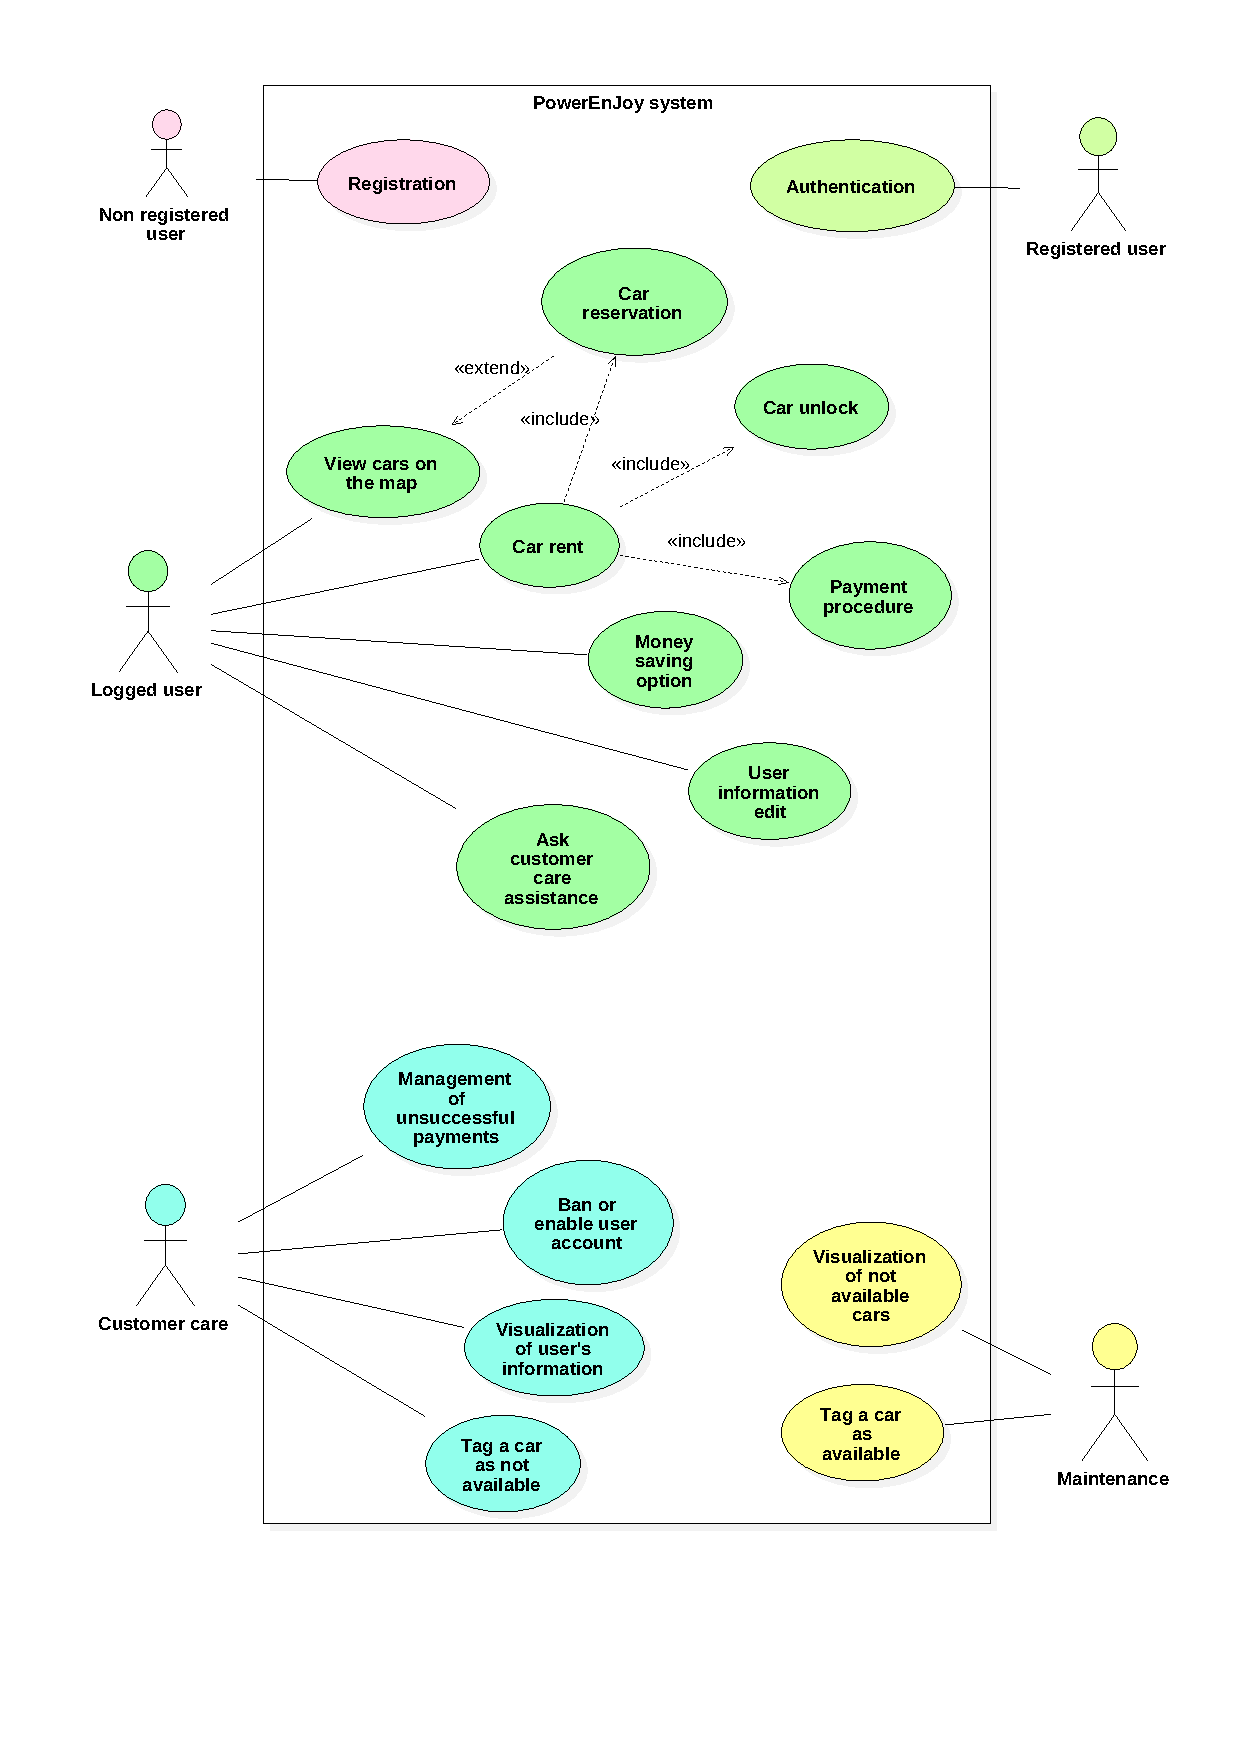
\includegraphics[width=0.9\textwidth]{useCase}
			\caption{
				\label{fig:useCase} 
				Use case diagram
			}
		\end{figure}
\subsection{Use cases description}

\begin{tabular}{p{0.25\linewidth}p{0.75\linewidth}}
\toprule
\textbf{Name} & \textbf{Registration} \\
\midrule
\textbf{Actors} & Non registered user \\
\midrule
\textbf{Entry conditions} & \\
\midrule
\textbf{Flow of events} & 
\begin{enumerate}
	\item The user asks the system to register to its services
	\item The system shows the appropriate form to fill to register to the system
	\item The user inserts an username to be uniquely identified by the system
	\item The user inserts his own email address
	\item The user inserts his name, surname, birth date and place and current domicile
	\item The user inserts his driving license ID code and expiring date
	\item The user inserts payment information
	\item The user confirms data inserted are correct e submit the form
	\item The system sends an email to the user with a unique link to verify the email address inserted by the user really belongs to him
	\item The user clicking on the link received confirms his email address
\end{enumerate} \\
\midrule
\textbf{Exit conditions} & The user is notified by mail the registration procedure is correctly completed and he is provided with a password bound to his username to access the system\\
\midrule
\textbf{Exceptions} & 
\begin{itemize}
	\item If the username inserted by the user is already used by another user, the system displays an error message asking the user to insert another username
	\item If the user doesn't receive the link sent to him by mail needs to complete the form again with a correct email address
	\item If the user notices to have entered wrong informations he could edit them at the end of the process of registration in his personal page
\end{itemize} \\
\bottomrule
\end{tabular}

\newpage

\begin{figure}[h]
			\centering
			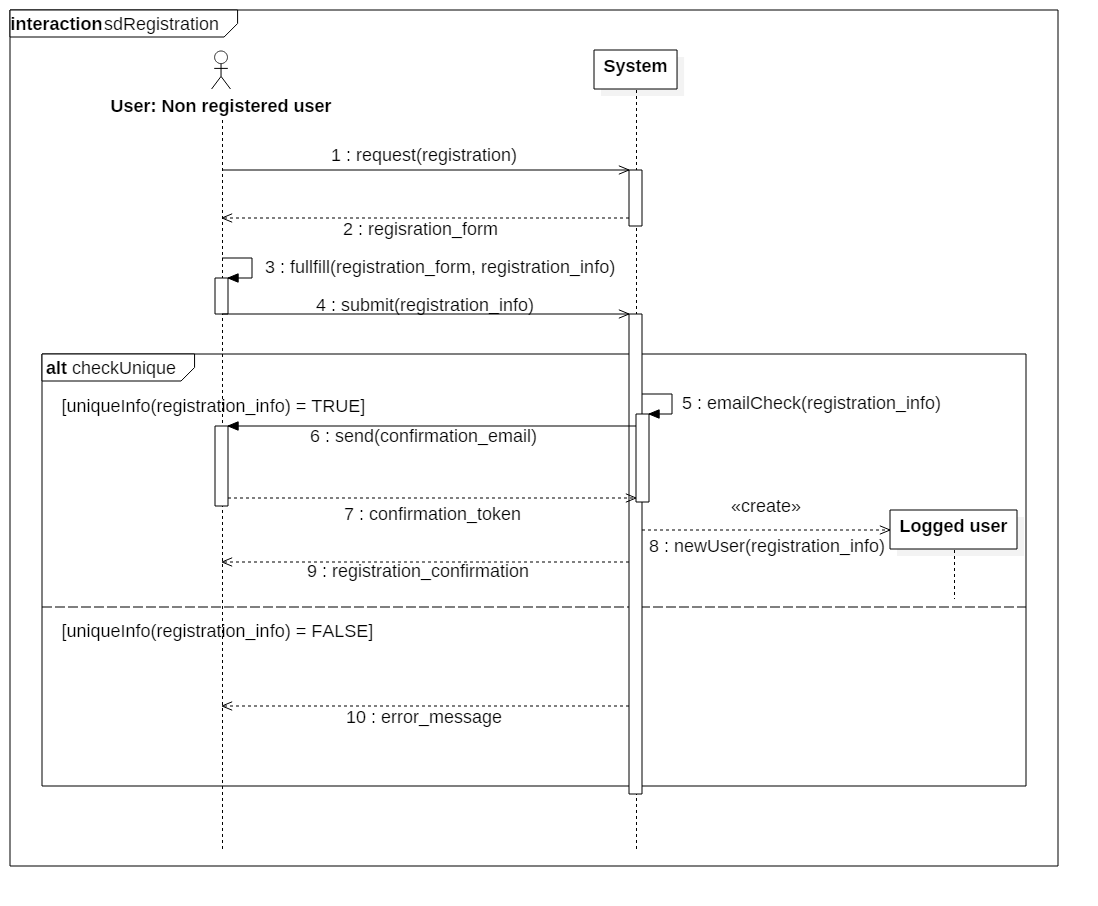
\includegraphics [width=\textwidth]{/diagrams/Sequence/sdRegistration.png}
			\caption{
				\label{fig:registrationSequence} 
				Registration sequence diagram
			}
		\end{figure}
		
\newpage
\begin{tabular}{p{0.25\linewidth}p{0.75\linewidth}}
\toprule
\textbf{Name} & \textbf{Authentication} \\
\midrule
\textbf{Actors} &  Registered user \\
\midrule
\textbf{Entry conditions} & The user must know his username and password \\
\midrule
\textbf{Flow of events} & 
\begin{enumerate}
	\item The user inserts his username and password in the appropriate form and submit it
	\item The system validates the inserted credential
	\item The system checks if the user is banned
\end{enumerate} \\
\midrule
\textbf{Exit conditions} & If the credential validation is successful and the user is not banned he is granted the proper privileges\\
\midrule
\textbf{Exceptions} & 
\begin{itemize}
	\item If the credential validation failed an error message is displayed
	\item If the credential validation is successful and the user is banned a message providing assistance is displayed and the system doesn't allows the user to access to the system
\end{itemize} \\
\bottomrule
\end{tabular}

\newpage

\begin{figure}[h]
			\centering
			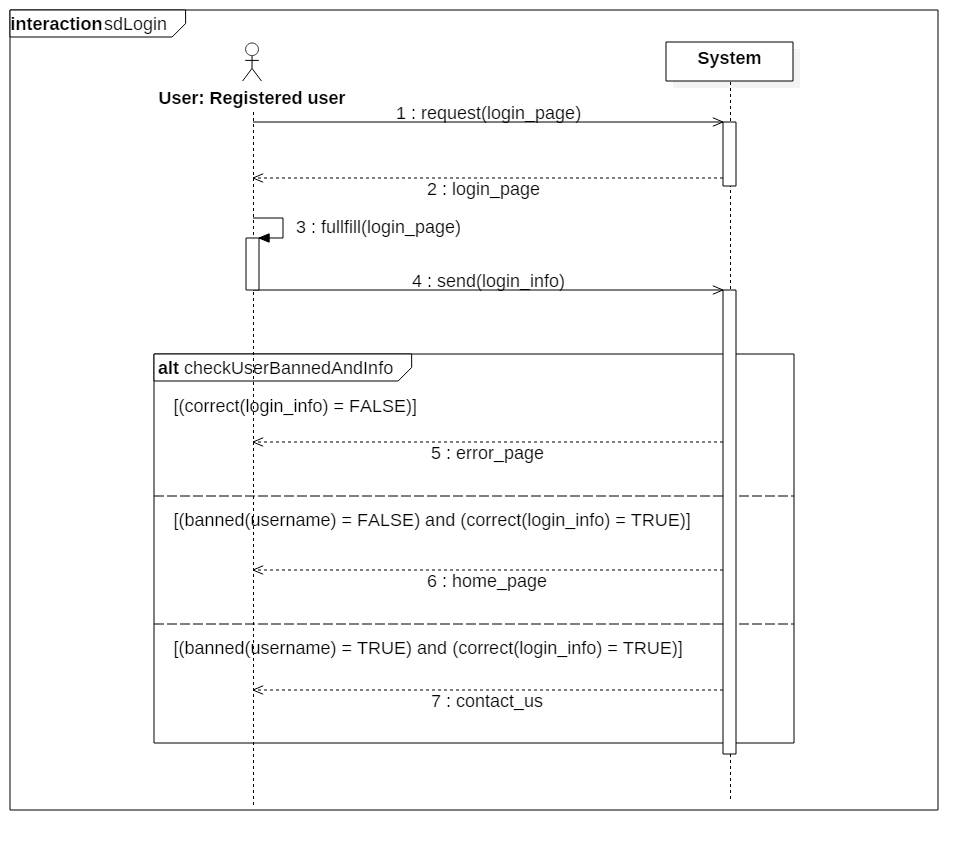
\includegraphics [width=\textwidth]{/diagrams/Sequence/sdLogin.png}
			\caption{
				\label{fig:authSequence} 
				Authentication sequence diagram
			}
		\end{figure}

\newpage

\begin{tabular}{p{0.25\linewidth}p{0.75\linewidth}}
\toprule
\textbf{Name} & \textbf{View cars on the map} \\
\midrule
\textbf{Actors} &  Logged user \\
\midrule
\textbf{Entry conditions} & \\
\midrule
\textbf{Flow of events} & 
\begin{enumerate}
	\item The user chooses if he wants to use his GPS position or insert a different one manually
		\subitem a. The system retrieves the user's GPS position
		\subitem b. The user inserts a position
	\item The system retrieves the position of all available cars and their battery level percentage
	\item The system shows a map with all available cars near the position indicated by the user
	\item The user can click on a car on the map to see its battery level percentage
\end{enumerate}\\
\midrule
\textbf{Exit conditions} & The user can navigate a map with all available cars near the position indicated by him\\
\midrule
\textbf{Exceptions} & 
If the position inserted by the user is not correct an error message is displayed \\
\bottomrule
\end{tabular}

\newpage

\begin{figure}[h]
			\centering
			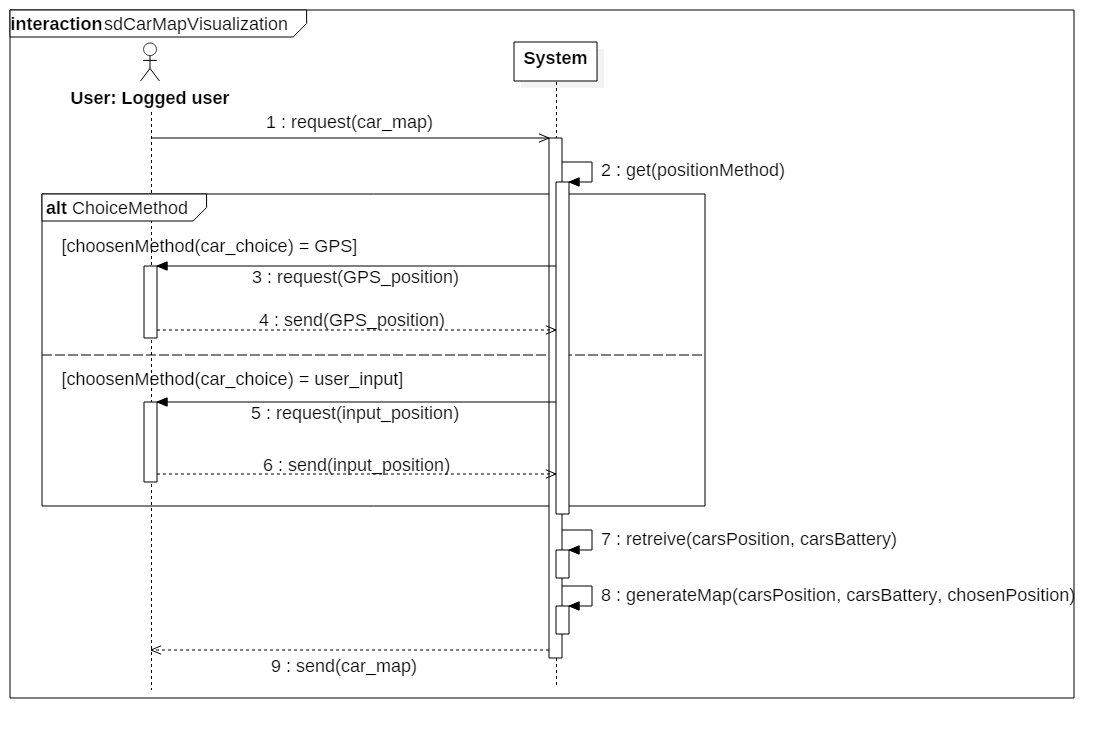
\includegraphics [width=\textwidth]{/diagrams/Sequence/sdCarMapVisualization.png}
			\caption{
				\label{fig:carsMapSequence} 
				View cars on the map sequence diagram
			}
		\end{figure}

\newpage

\todo{Car reservation punto 2: retrieves->refresh}
\begin{tabular}{p{0.25\linewidth}p{0.75\linewidth}}
\toprule
\textbf{Name} & \textbf{Car reservation} \\
\midrule
\textbf{Actors} &  Logged user \\
\midrule
\textbf{Entry conditions} & \\
\midrule
\textbf{Flow of events} & 
\begin{enumerate}
	\item \emph{View cars on the map}
	\item The user selects the car he wants to reserve
	\item The user confirms he wants to reserve that car
\end{enumerate}\\
\midrule
\textbf{Exit conditions} & The system set the state of the chosen car as \emph{Reserved} paired with the user who made the reservation\\
\midrule
\textbf{Exceptions} &  If the user has already reserved a car, the system shows an error message and doesn't allow him to reserve another car \\
\bottomrule
\end{tabular}

\begin{tabular}{p{0.25\linewidth}p{0.75\linewidth}}
\toprule
\textbf{Name} & \textbf{Car unlock} \\
\midrule
\textbf{Actors} &  Logged user \\
\midrule
\textbf{Entry conditions} & The user should have done a reservation for a car \\
\midrule
\textbf{Flow of events} & 
\begin{enumerate}
	\item The user select the unlock button to ask the system to unlock the car
	\item The system checks if the user's position is at most 5 meters away from the position the car he reserved
	\item The system unlocks the car
\end{enumerate} \\
\midrule
\textbf{Exit conditions} & The car is unlocked and the user may enter it\\
\midrule
\textbf{Exceptions} & 
\begin{itemize}
	\item If the user credentials doesn't correspond to the credential of the user paired with the \emph{Reserved} state of the car the system displays an error message
	\item If the position of the user is not at most 5 meters away from the position the car he reserved the system displays an error message
\end{itemize} \\
\bottomrule
\end{tabular}

\todo{Car Rent: corsivo=UC || Glossary ? Perchè specificare notifica EMAIL?}
\begin{tabular}{p{0.25\linewidth}p{0.75\linewidth}}
\toprule
\textbf{Name} & \textbf{Car Rent} \\
\midrule
\textbf{Actors} &  Logged user \\
\midrule
\textbf{Entry conditions} & \\
\midrule
\textbf{Flow of events} & 
\begin{enumerate}
	\item \emph{Car reservation}
	\item \emph{Car unlock}
	\item The user ignites the car engine
	\item The system sets the state of the \emph{Reserved} car to \emph{In Use} paired
	with the same user
	\item During the rent the user is informed about the current charge and if it is or not inside a
	safe area
	\item The user leaves the auto turning off the engine
	\item The system locks the car
    \item The system activates a timer to allow the user to plug the car into a power grid if it is
    near one of them
	\item When the timer expires: \emph{Payment procedure}
	\item The system sets the car as \emph{Available}
\end{enumerate} \\
\midrule
\textbf{Exit conditions} & 
The user is charged of the correct amount for the ride and at anytime could perform another rent, the car is available again\\
\midrule
\textbf{Exceptions} & 
\begin{itemize}
	\item If the user doesn't start the engine up to one hour after the reservation, he is charged of 1\euro , the car state is set as \emph{Available} and the user is notified by email his reservation is expired
	\item ...
\end{itemize} \\
\bottomrule
\end{tabular}
\begin{tabular}{p{0.25\linewidth}p{0.75\linewidth}}
\toprule
\textbf{Name} & \textbf{Payment procedure} \\
\midrule
\textbf{Actors} &  Logged user\\
\midrule
\textbf{Entry conditions} & 
The user must have completed a rent shutting off the engine and exiting the car. The timer activated by the system locking the car expires. \\
\midrule
\textbf{Flow of events} & 
\begin{enumerate}
	\item The system checks if the car position is or is not inside a safe area
	\item The system checks if the car has detected more then one passenger during the rent
	\item The system checks the car battery percentage
	\item The system checks if the car is plugged on a charging station
	\item The system checks the distance of the car from the nearest charging station
	\item The system calculates the cost of the ride based on the rent time
	\item The system determines the applicable discounts/extra fee applying it to the cost of the ride
	\item The system starts a payment procedure with user's payment information using
	an external service
	\item The system waits a response from the external payment service
	\item The system logs data about the rent and the payment
    \item The system notifies through email the user about the result of the payment procedure and on discount/extra fees applied
\end{enumerate} \\
\midrule
\end{tabular}

\begin{tabular}{p{0.25\linewidth}p{0.75\linewidth}}
\midrule
\textbf{Alternative flow} & 
Flow of events as specified upon from \emph{1} to \emph{7}
\begin{enumerate}[label=8 \alph*.]
	\item The system detects the user has enabled the \emph{money saving option}
	\item The system checks if the car is currently on charge on the charge station determined by the system at the begin of the rent
	\item The system determines the applicable discounts/extra fee applying it to the cost of the ride eventually also taking in account the \emph{money saving option} discount if the car is currently on charge on the charge station determined by the system at the begin of the rent
\end{enumerate}
Flow of events as specified upon from \emph{9} to \emph{12} \\
\midrule
\textbf{Exit conditions} & 
The user is charged of the correct amount for the ride\\
\midrule
\textbf{Exceptions} & 
\begin{itemize}
	\item If the payment procedure is not correctly completed because of insufficient credit the user is banned, rent information is stored, the payment suspended and the user is informed through mail to contact the customer service.  
	\item ...
\end{itemize} \\
\bottomrule
\end{tabular}

\begin{tabular}{p{0.25\linewidth}p{0.75\linewidth}}
\toprule
\textbf{Name} & \textbf{Money saving option} \\
\midrule
\textbf{Actors} &  Logged user\\
\midrule
\textbf{Entry conditions} & 
The user should have enabled the \emph{money saving option} \\
\midrule
\textbf{Flow of events} & 
\begin{enumerate}
	\item \emph{Car Reservation}
	\item The system asks the user to insert his destination
	\item The user inserts his destination
	\item The system searches for charging stations near the destination position inserted by the
	user with available plugs
	\item The system chooses a charging station in order to ensure a uniform distribution of cars in
	the city and taking in account the destination of the user
	\item The system informs the user about the charging station to reach in order to obtain the discount
	\item \emph{Car Rent} (\emph{Car Reservation} already done)
\end{enumerate} \\
\midrule
\textbf{Exit conditions} &
\begin{itemize}
	\item If the user has left the car plugged in the charging station suggested by the
	\emph{money saving option} he has obtained the correct discount
	\item The user can  anytime ìperform another rent
	\item Car is again available
\end{itemize} \\
\midrule
\textbf{Exceptions} & 
\begin{itemize}
	\item If the user doesn't leave the car in the charging station suggested by the
	\emph{money saving option} he doesn't obtain the related discount
	\item ...
\end{itemize} \\
\bottomrule
\end{tabular}

\begin{appendices}

	\section{Alloy model}
		\subsection{Source code}
		\lstinputlisting[language=alloy]{alloy/alloy2.0version.als}
		\begin{figure}[h!]
			\centering
			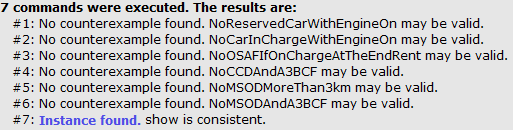
\includegraphics[]{alloy/AlloyResult.png}
			\caption{
				\label{fig:alloyExecutionResult} 
				Alloy execution result
			}
		\end{figure}
		\clearpage
		\subsection{Generated worlds}
			Note that in \autoref{fig:alloyWorld1} LoggedUser3 has been banned \emph{after} completing RentMade0.
			\begin{figure}[h!]
			\centering
			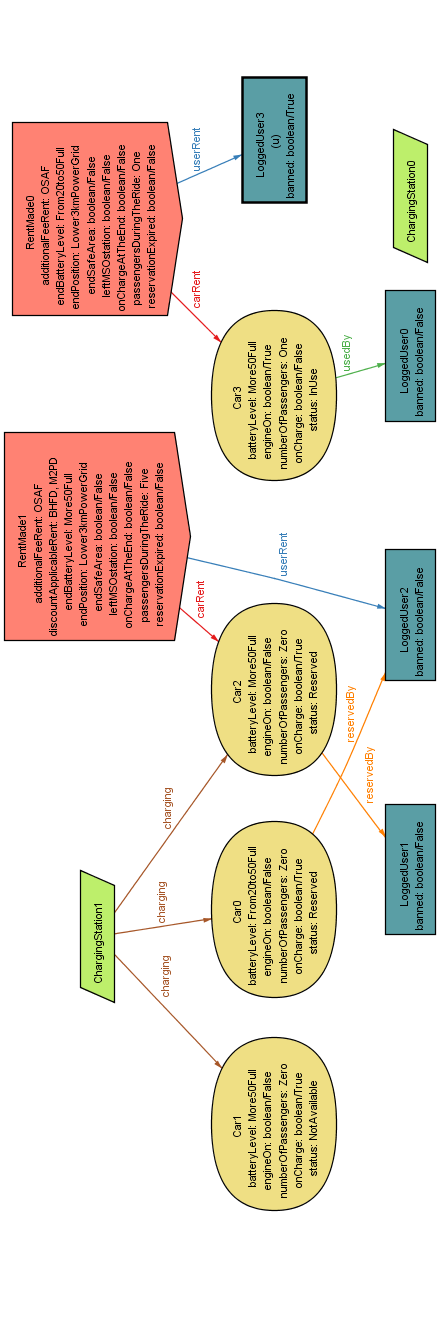
\includegraphics[scale=0.39]{alloy/AlloyWorld2.png}
			\caption{
				\label{fig:alloyWorld1} 
				First alloy generated world
			}
		\end{figure}
		\clearpage
		Note that in \autoref{fig:alloyWorld2} RentMade1 is actually a reservation expired of Car3 made by LoggedUser2. He now has reserved Car1.
		\begin{figure}[h!]
		\centering
		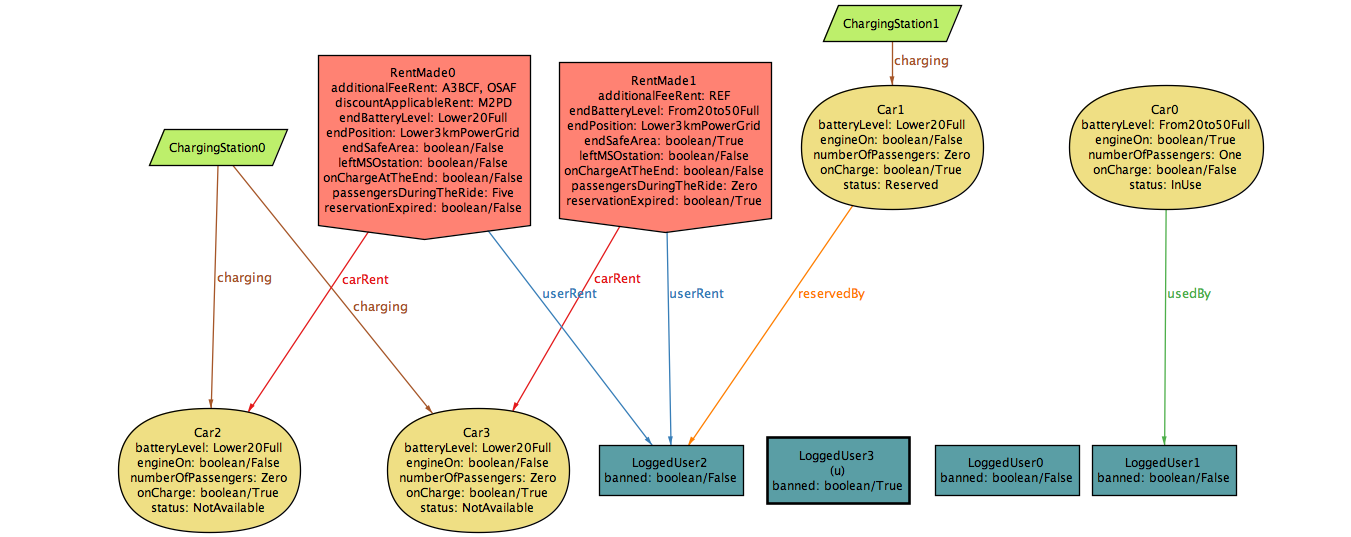
\includegraphics[scale=0.39]{alloy/AlloyWorld1.png}
		\caption{
			\label{fig:alloyWorld2} 
			Second alloy generated world
		}
		\end{figure}
		\clearpage
	\section{Software and tools used}
	For the development of this document we used
	\begin{itemize}
		\item \LaTeX{} as document preparation system
		\item Git \& \href{http://github.com}{GitHub} as version control system
		\item \href{http://draw.io}{Draw.io} for graphs
		\item StarUML for diagrams
		\item Alloy as model analyzer
	\end{itemize}
	
	\section{Hours of work}
	This is the team members' effort spent to redact this document:
	\begin{itemize}
		\item Davide Piantella: $\sim$ 48 hours
		\item Mario Scrocca: $\sim$ 48 hours
		\item Moreno R. Vendra: $\sim$ 45 hours
	\end{itemize}
\end{appendices}
\clearpage
\begin{thebibliography}{9}
\bibitem{RE}B. Nuseibeh, S. Easterbrook, \emph{Requirements Engineering: A Roadmap}, 2000
\bibitem{Zave}P. Zave, \emph{Classification of Research Efforts in Requirements
Engineering}, ACM Computing Surveys, 1997
\bibitem{Assignments} E. Di Nitto, L. Mottola, \emph{Assignments Software Engineering 2}, AA 2016-2017
\bibitem{IeeeRasd}IEEE Std 830:1993, \emph{IEEE Recommended Practice for Software Requirements Specifications}, 1993
\bibitem{WorldMachine}M. Jackson, \emph{The World and the Machine}, 1995
\bibitem{TextualAnalysis}R. J. Abbot, \emph{Textual (noun-verb) analysis},1983
\end{thebibliography}

\end{document}
